\section{Evaluation and Results}

We sample 1000 graphs from each model and evaluate novelty (fraction not isomorphic to any training graph), uniqueness (fraction with no duplicate in the sample), and their intersection. Isomorphism is checked via the Weisfeiler-Lehman graph hash~\cite{shervashidze2011weisfeiler}.

\begin{center}
\small
\begin{tabular}{lccc}
\toprule
 & Novel & Unique & Novel+Unique \\
\midrule
Baseline  & 100\% & 100\% & 100\% \\
GraphVAE  & 100\% & 100\% & 100\% \\
\bottomrule
\end{tabular}
\captionof{table}{Novelty and uniqueness over 1000 samples.}
\label{tab:novelty}
\end{center}

Both models score 100\% across the board. This is expected rather than impressive: the combinatorial graph space is enormous, so random sampling almost never revisits a training graph or produces a duplicate.

\autoref{fig:histograms} compares node degree, clustering coefficient, and eigenvector centrality across the empirical distribution, the baseline, and GraphVAE. The baseline matches the empirical degree distribution more closely than GraphVAE, but it still diverges on clustering because it only matches edge density per $N$. GraphVAE overshoots on all three statistics: generated graphs are denser than real ones, which increases clustering and shifts the centrality distribution.

\begin{center}

\includegraphics[width=\linewidth]{../outputs/evaluation/2026-05-06_12-20-00/histogram_grid.pdf}
\captionof{figure}{Graph statistics for the empirical distribution (left), Erdős-Rényi baseline (centre), and GraphVAE (right). Bins are shared within each row.}
\label{fig:histograms}
\end{center}

\autoref{fig:samples} makes this concrete. Real MUTAG graphs are sparse, and GraphVAE samples have about 1.6--3.1$\times$ more edges than training graphs at the same node count (median $\sim$2.3$\times$), so the decoder has not learned the low edge density of molecular graphs.

\begin{center}
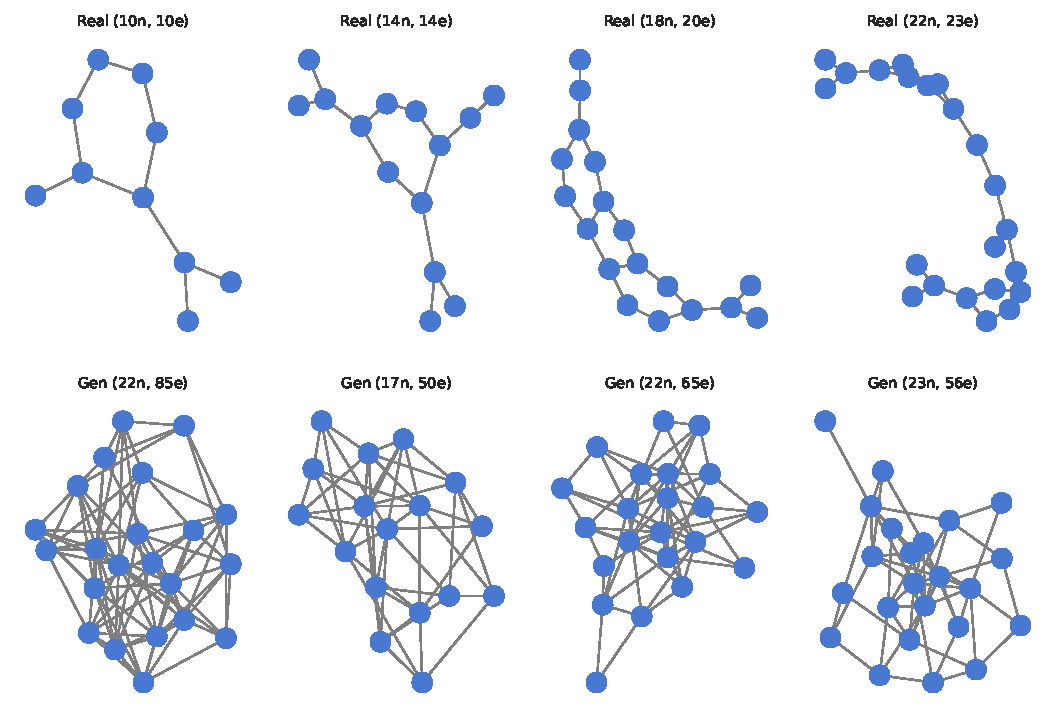
\includegraphics[width=\linewidth]{../outputs/train_gvae/2026-05-06_11-54-12/sample_grid.pdf}
\captionof{figure}{Four real MUTAG graphs (top) and four GraphVAE samples (bottom) with node/edge counts.}
\label{fig:samples}
\end{center}
